\section{DeepFaceLive}\label{sec:deepfacelive}
\gls{dflive} ist ein weiteres Open-Source-Tool zur Erstellung von Deepfakes, das sich auf Echtzeitanwendungen konzentriert.
Es ermöglicht die nahtlose Integration von Gesichtsaustausch in Video-Streams, was die Software für Social Engineering interessant macht.

\subsection{Motivation}\label{subsec:motivation_dflive}
Die Hauptmotivation hinter \gls{dflive} ist es, die Möglichkeiten der Echtzeit-Gesichtsmanipulation zu erforschen und zu erweitern.
Dadurch wird es möglich, Gesichter in Videos während des Streamings in Echtzeit auszutauschen, was neue Anwendungen und Herausforderungen sowohl im Bereich der Unterhaltung als auch der Sicherheit mit sich bringt.

\subsection{Fähigkeiten}\label{subsec:fahigkeiten_dflive}
\begin{itemize}
    \item \textbf{Reenactment von Bildern:} Schneller und einfach, bei gutem Ausgangsbild akzeptable Ergebnisse
    \item \textbf{Face Swapping mit Bildern:} Schneller und einfach, bei gutem Ausgangsbild akzeptable Ergebnisse
    \item \textbf{Face Swapping eines DFM Modells:} Erfordert Modelltraining in \gls{dfl}, dafür bessere Ergebnisse
\end{itemize}

\subsection{Workflow}\label{subsec:workflow_dflive}
Der Workflow von DeepFaceLive umfasst mehrere Schritte, um eine nahtlose Echtzeit-Gesichtsmanipulation zu gewährleisten:

\subsubsection*{Initialisierung}\label{subsubsec:initialisierung_dflive}
Die Initialisierung umfasst das Einrichten der Umgebung und das Laden der notwendigen Modelle.
Nutzer können Modelle aus dem Internet verwenden oder eigene Modelle trainieren, um spezifische Anforderungen zu erfüllen.
Die Pipeline von \gls{dflive} besteht aus mehreren Schritten.\\

\subsubsection*{Data Source}
Das \texttt{dst}-Video kann entweder per Datei oder als Kamera-Stream bereitgestellt werden.
Das Verwenden einer Datei hat im Kontext von Social Engineering allerdings keine Relevanz.

\subsubsection*{Detection, Alignment and Marking}
Der nächste Schritt ist das Erkennen von Gesichtern im Ausgangsmaterial.
Hierfür stehen verschiedene Algorithmen bzw. Neuronalen Netze zur Verfügung: CenterFace, S3FD oder YoloV5.
Das erkannte Gesicht wird anschließend mittig im Bild ausgerichtet und mit Landmarks markiert.
Auch für diesen Schritt stehen verschiedene Möglichkeiten zur Verfügung: OpenCV LBF, Google FaceMesh oder InsightFace\_2D106.
Die Standardeinstellungen sind in den meisten Fällen ausreichend, ggf. können auch andere Modelle getestet werden.

\subsubsection*{Face Swapping/Reenactment}
Nachdem das \texttt{dst}-Material nun für den Tausch vorbereitet wurde kann zwischen drei Möglichkeiten gewählt werden.
\textbf{Face animator} bietet die Möglichkeit des Reenactments eines Bildes.
Dafür ist es empfehlenswert ein gut belichtetes, neutrales Bild zu verwenden.
Diese Variante ist für Social Engineering Angriffe bedingt geeignet.
Nutzt man die Technik und legt im Nachhinein flasche Störsignale über das Video, werden die Nachteile dieses einfachen Modells überdeckt.
Diese Art kann also nur in Video-Chats verwendet werden.
\begin{figure}[h]
    \center
    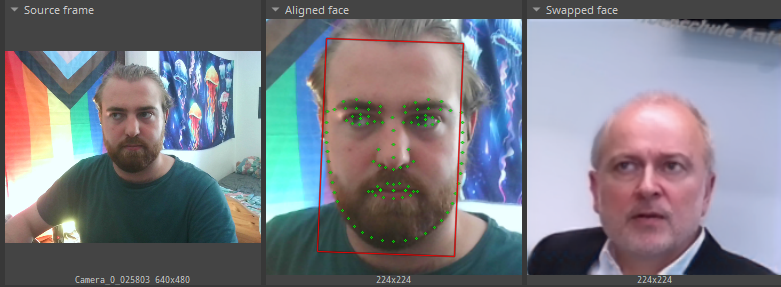
\includegraphics[width=0.7\textwidth]{Bilder/DFLive/face-animator}
    \caption{Face Animator Pipeline}
    \label{fig:dflive-reenactment}
\end{figure}

\textbf{Face swap (Insight)} bietet die Möglichkeit ein Gesicht aus einem einzelnen Bild auf ein Zielgesicht zu swappen.
Hier ist die Qualität des Bildes ebenfalls entscheidend.
\begin{figure}[h]
    \center
    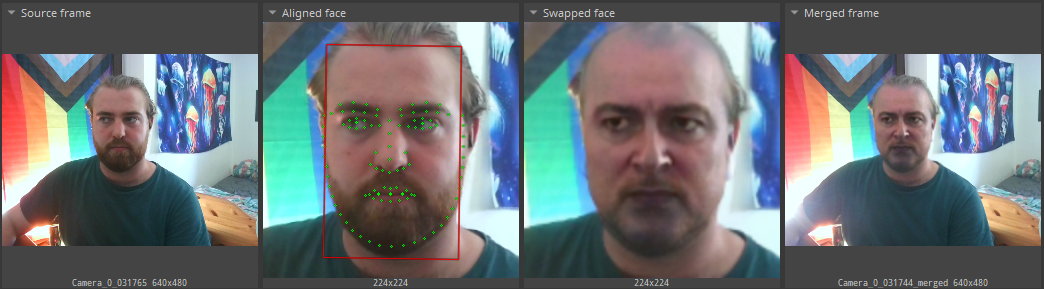
\includegraphics[width=0.7\textwidth]{Bilder/DFLive/Face-swap-ingsight}
    \caption{Face Swap (Insight)}
    \label{fig:dflive-insight-swapping}
\end{figure}

\textbf{Face swap (DFM)} benutzt in DeepFaceLab (DFL) trainierte Modelle zum Ersetzen der Gesichter.
Dies bietet den Vorteil, das das Gesicht (bei richtigem Training) von verschiedenen Blickwinkeln und Expressionen richtig dargestellt wird.
Die Ergebnisse sind natürlicher als die, die nur auf einem Bild basieren.
Allerdings fordert diese Variante einen deutlich höheren Mehraufwand. 
Es müssen zuerst genügend Bilder zusammengetragen werden und ein Modell trainiert werden.
Außerdem muss beim Face swap eine Person, die ähnlich wie die Zielperson aussieht den Deepfake bzw. Social Engineering Angriff durchführen.
% TODO Bild von fertigem Modell

\subsubsection*{Face Merger und Output}
Wird ein Gesicht getauscht, muss das Zielgesicht wieder mit dem Originalbild zusammengefügt werden.
Diese aufgabe übernimmt der \texttt{Face Merger}, hier können ebenfalls verschiedene Einstellungen geändert werden, die aus \gls{dfl} bekannt sind.
Für Reenactment ist dies nicht nötig.
Anschließend kann der modifizierte Video-Stream entweder in einer Datei gespeichert werden, per \texttt{mpegts udp} gestreamt oder in einem neuen Fenster angezeigt werden.
Durch Tools wie die \gls{obs} kann dieses Fenster wiederrum als virtuelle Kamera in anderen Anwendungen verwendet werden.

\subsubsection*{RTT Model Training}
Das Trainieren eins \gls{rtt} Models, weicht von der in Kapitel \ref{sec:praxisbeispiel-dfl} beschriebenen Methode ab.
Im wesentlichen Unterscheiden sich die zum Training verwendeten Datensätze.
Für ein \gls{rtt} Model muss das Gesicht das später als \texttt{.dfm}-Datei in \gls{dflive} verwendet werden soll gewohnt als \texttt{src} verwendet werden.
Dieses Mal wird das Modell allerdings nicht auf ein Zielgesicht, sondern auf möglichst viele verschiedene Gesichter trainiert.
Dafür sind entsprechende \gls{rtt} Facepacks im Internet zu finden.
Pretrained Models können allerdings trotzdem verwendet werden.
Sonst folgt der Workflow dem in Abschnitt \ref{sec:praxisbeispiel-dfl} beschriebenen.